% PGF text plot marks in a mathematical coordinate system.
\documentclass[border=2pt]{standalone}
\usepackage{pgfplots}
\usetikzlibrary{plotmarks}
\pgfplotsset{compat=newest}

\begin{document}
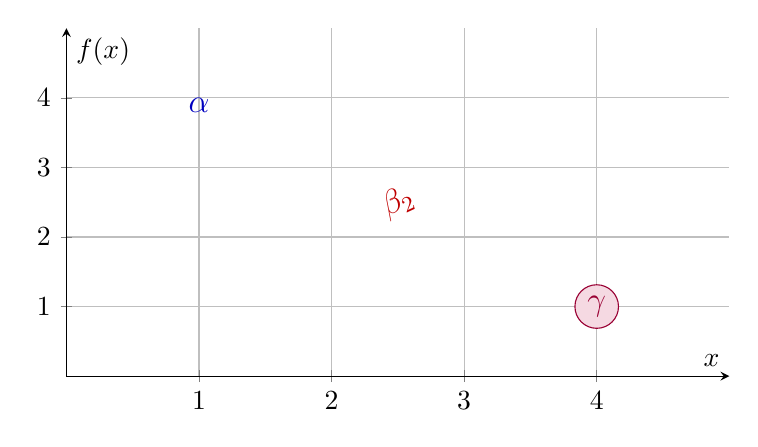
\begin{tikzpicture}
  \begin{axis}[
    width=10cm,height=6cm,
    xmin=0,xmax=5,ymin=0,ymax=5,
    axis lines=middle,grid=major,
    xlabel={$x$},ylabel={$f(x)$},
    xtick={1,2,3,4},ytick={1,2,3,4}
  ]
    \addplot[only marks,blue!75!black,mark=text,
      text mark={{\large$\alpha$}},text mark style={top}]
      coordinates {(1,4)};
    \addplot[only marks,red!75!black,mark=text,
      text mark={{\large$\beta_2$}},text mark style={rotate=25}]
      coordinates {(2.5,2.5)};
    \addplot[only marks,purple!80!black,mark=text,
      text mark={$\gamma$},text mark as node=true,
      text mark style={draw,fill=purple!15,circle,inner sep=2pt,font=\large}]
      coordinates {(4,1)};
  \end{axis}
\end{tikzpicture}
\end{document}
